\documentclass[12pt,a4paper,oneside]{article}
%\documentclass[12pt,a4paper,oneside,twocolumn]{article}
\usepackage{pagestyle}
\usepackage{codestyle}

% Report hand-in date
\DTMsavedate{date}{2024-03-29}

\title{
    \Huge{Machine Learning} \\ \LARGE 
    Nature's Quest: Deep Learning Exploration of Global Plant Traits from Images and Geodata
}
\author{
Kai E. Niermann \and
Dávid Miklo \and 
Trix Taicet \and
Red Kaláb \and
Conner Dassen
}
\date{\DTMusedate{date}}
\begin{document}
\maketitle

% \lstinputlisting[firstline=10, lastline=13]{code/sample_script.py}

\begin{abstract}
    % Abstract content goes here
\end{abstract}

\section{Introduction}
% primary paragraph 
Global warming and more broadly climate change have become a major concern for the world as its effects are becoming more and more apparent \cite{WANG2023100237}. Changing weather patterns, especially towards more extreme conditions are causing plants to adapt to new environments \cite{GRAY201664}. One method of measuring said adaptation is to look at the traits, that is, properties of a plant that describe how it functions and interacts with the environment. These traits include but are not limited to the plant height, leaf area, but also dry mass, and leaf nitrogen content amongst various others. Monitoring these traits allows us to gain vital insights into how climate change impacts different ecosystems. While somewhat simple manual measurement techniques exist, at scale they are not feasible. This is where Convolutional Neural Networks (CNN) come in.  

\smallskip
Through the work demonstrated by Schiller et al \cite{schiller2021deep} we know that CNNs can be used to predict plant traits from images. The images used to train this network came from \textit{citizen science photographs} which are images taken by citizens of plants from all across the world using AI plant species identification apps (e.g. iNaturalist, Pl@ntNet). Citizen science photographs also come with location metadata, which can be used to extract ancillary geodata such as precipitation, temperature, and soil type. This geodata can optionally be combined with the images to create a CNN which can potentially learn to extract features from images in conjunction with geodata to predict plant traits.

\smallskip
For our method, we wanted to compare the accuracy of a CNN trained on images alone and using a pre-trained backbone (e.g. ResNet, EfficientNet, etc.) to a CNN trained on images and geodata. We hypothesize that the CNN trained on images and geodata will outperform the CNN trained on images alone. With our results we hope to provide a better understanding of the key factors that are needed to predict plant traits.

% secondary paragraph
% \section{Literature review}

\section{Method}

\subsection{Data processing}

Integral to any machine learning model is the data used to train, validate, and ultimately test the model. The data used consisted of 3 main components: ancillary geodata from various sources, the main task trait means and auxiliary task standard deviations, and the training ima ges of the plants.

\smallskip 
Upon visual inspection one of the first issues we spotted was a considerable chunk (29.53\%) of data missing for the auxiliary task standard deviations. Through some previous work on the same Kaggle, we noticed that the auxiliary data was a useful inclusion. We can also validate these reports with previous work applying auxiliary tasks in CNNs such as the work of Lukas Libel and Marco Kroener which found that the inclusion of an auxiliary task with minor relevance to the main task did indeed boost performance \cite{lukaslibel} and Chen et. al. \cite{pmlr-v80-chen18a} which demonstrated that for very similar or mostly similar auxiliary tasks the contribution is generally a positive one. Based on this we decided to use a simple k-nearest neighbor (kNN) imputation strategy which has generally proved effective \cite{joel2024performance}. The rest of the data had all values present.

\smallskip
The geodata was another point of consideration in the data pre-processing phase. Looking at the individual columns we noticed that the instances had features that encoded similar information and thus were likely redundant in the training process. Since we are working with a very high dimensional feature space to get some sort of visual verification of this claim we plotted a correlation heatmap for the 3 biggest groups of the geodata, namely the datasets: SOIL, MODIS, and VOD.

\begin{figure}[!h]
    \centering
    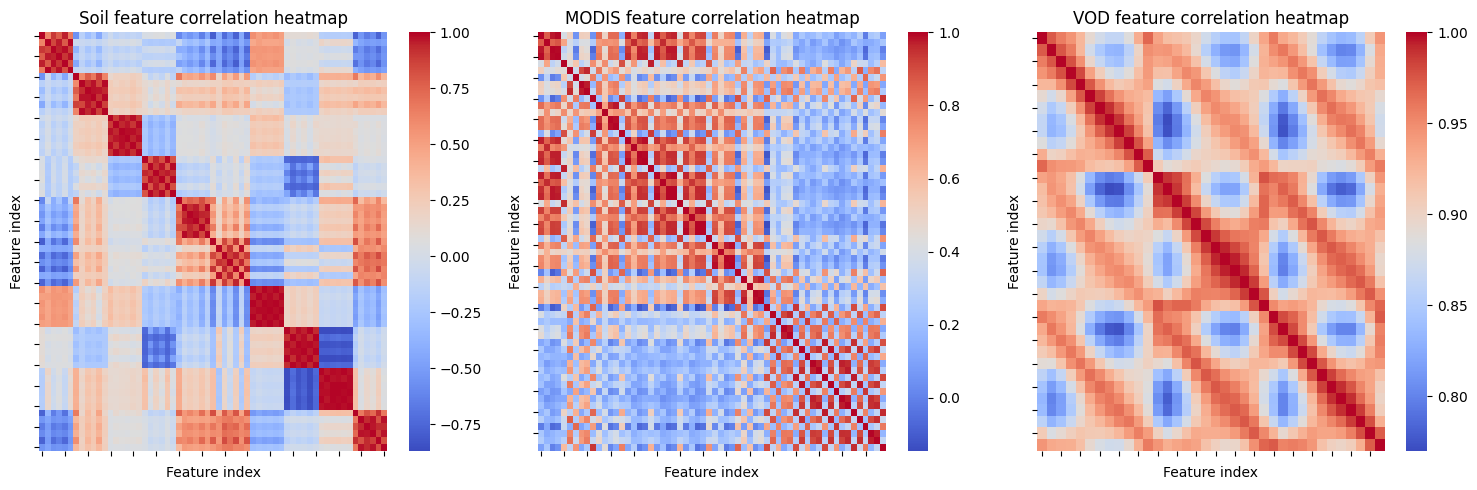
\includegraphics[width=0.9\textwidth]{assets/corr_hm.png}
    \caption{Correlation heatmap of the 3 biggest groups of geodata}
\end{figure}

Since these datasets individually can be broken down into groups of features generally talking about a similar topic (e.g. precipitation metrics, temperature metrics, etc) we can see that the correlation within these groups is quite high. Even though previous work \cite{DBLP:journals/corr/abs-2007-00062} has demonstrated the viability of neural network models to learn from high dimensional data, removing redundant features has in numerous instances been shown to improve model performance \cite{chen2022survey}. With this in mind, we decided to apply a Principal Component Analysis (PCA) to the geodata to reduce the dimensionality of the data. We specified that the number of principal components should be such that 95\% of the variance is explained.  

\subsection{Data preparation}

% talk about the augmentation 
Our training and test image instance - consisting of science citizen photographs - were taken by a wide variety of people under a wide variety of conditions. This means that the images are of varying quality, resolution, and orientation. We can see this just by taking a random sample of 5 images.
\begin{figure}[!h]
    \centering
    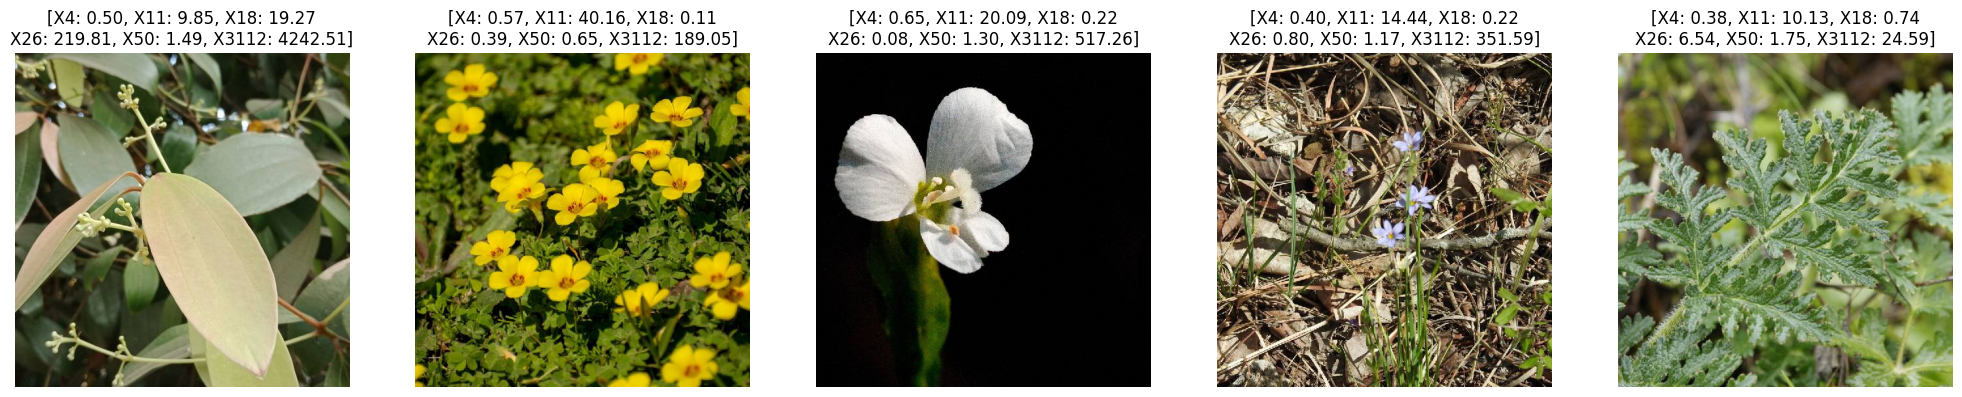
\includegraphics[width=0.9\textwidth]{assets/before_aug_img.png}
    \caption{Random sample of 5 images before augmentation annotated with their target trait labels}
\end{figure}

To prevent our model from fitting to noise in the data as a byproduct of how images were taken we decided to apply different keras preprocessing layers to batches concurrently. A key benefit of this would be that the model can generalize better to unseen data by learning potentially more meaningful features. While this approach of applying augmentations in the preprocessing stage is less flexible than having filters integrated into the model it does reduce model complexity though at the cost of potentially losing some ability to learn more complex features by being able to dynamically adjust the filters. Sampling again we can look at the results of our augmentations. 

\begin{figure}[!h]
    \centering
    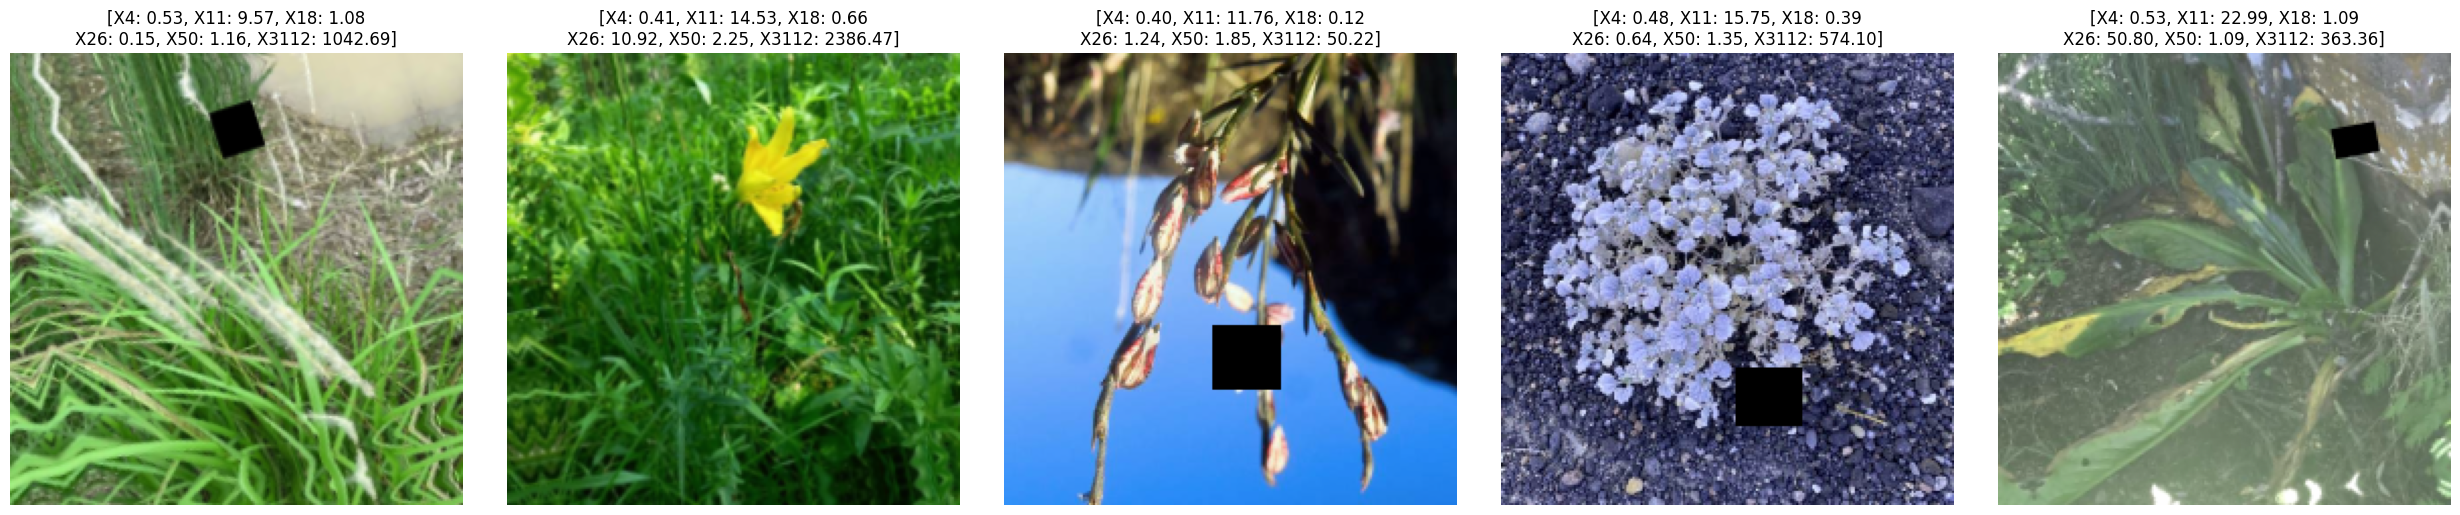
\includegraphics[width=0.9\textwidth]{assets/after_aug_img.png}
    \caption{Random sample of 5 images with augmentations: brightness, rotation, contrast, zoom, hue, cutout, flip, blur, saturation}
\end{figure}

% 5-fold stratified cross-validation + verification and split 
% \cite{Marcot2021} k = 5 good for large sample
% \cite{kequal10isgood} k ~ 10 generally good choice

\smallskip 
In addition to augmentation we noted that - though not too common - there was still a presence of certain substantial outliers in our data. Through visual inspection a common reason seems to have been specifically how close an indivdiual was when they took an image. As the training data itself was labelled by a machine learning model in a supervised fashion its evident perspective was not something the intial model had learned. As this scaling issue is a byproduct of the inital model which labelled the data and not any true property of the data we decided to remove these outliers. We did this by constraining the target distributions to the interval $[0.0001, 0.9999]$ and then removing any instances that were outside of this interval.

\smallskip
Another method of reducing overfitting we thought relevant to apply here would be k-fold cross-validation for the data split. We chose $k=5$ as for large datasets this has proven effective \cite{Marcot2021} and is generally around the commonly chosen value of 10 \cite{kequal10isgood}, where the 0th fold was designated as the validation set. Given that the data is from a geographically large enough sample we decided to create the folds in a stratified manner under the assumption the distribution of traits would be reasonably representative of the true distribution and thus one the model should learn. This is important as it ensures that the model is trained on a representative sample of the data in each fold and in turn, has its predictions distributed in a similar manner to the assumed true distribution of the traits. So we reduce the risk of overfitting to the training data while also ensuring the model is trained using a representative sample of targets in each fold. To validate that the distributions of the target traits are indeed similar we averaged the distributions of the target traits in each fold overlayed this on the original distribution of trait means and normalized them to the same scale.  

\begin{figure}[!h]
    \centering
    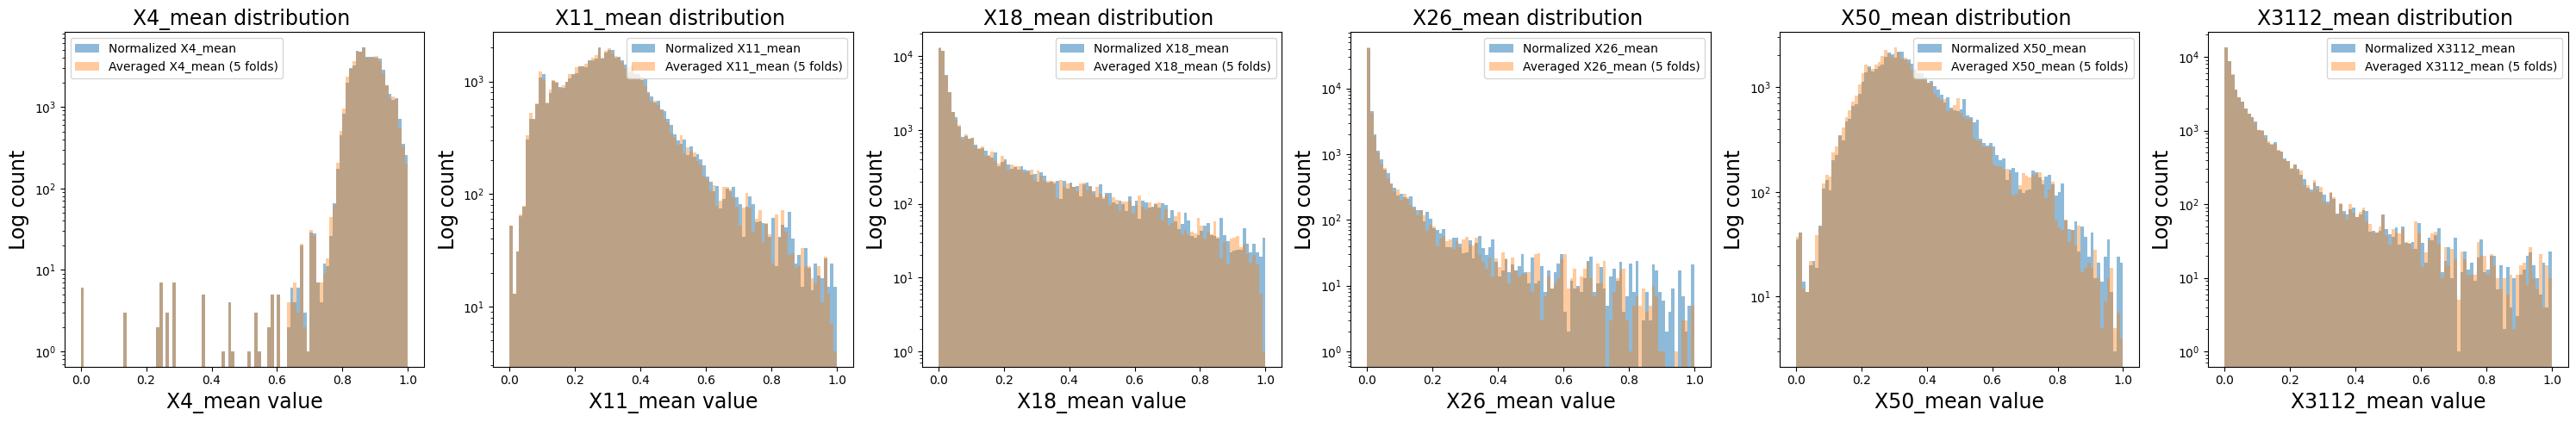
\includegraphics[width=1\textwidth]{assets/distribution_match_folds.png}
    \caption{Comparison of the average trait distributions in each fold with the original distribution of trait means ; (blue) normalized distribution of the trait means across the entire dataset ; (yellow) average normalized distribution of the trait means in each fold}
\end{figure}

\subsection{Model design}

\subsubsection{CNN trained on images}

% give an overview of the model 
    % activation function 
    % batch size
    % optimizer 
    % epochs
Our image CNN is a multi-output model that takes in a tensor consisting of red, green, and blue channels with an image size of 224x224 pixels. The model consists of a trained backbone; in our instance, we compared \textit{efficientnetv2\_b2\_imagenet}, \textit{efficientnetv2\_s\_imagenet}, and \textit{resnet50\_imagenet}. The backbone outputs then feed into a global average pooling layer, followed by 2 dense layers and a dropout layer connected to the two dense output layers for the main and auxiliary tasks. The hidden layers use a ReLU activation function, the outputs use no activation function as the targets are continuous. The model is trained using the Adam optimizer with a learning rate of 1e-4, a batch size of 48, and for 12 epochs. Additionally, we used the $R^2$ metric for both loss and evaluation of the model performance as this is a regression problem. Finally, we used step-based for the learning rate schedule which was defined as follows
\[
    \text{lr} = \text{lr}_\text{max} \times d^{\floor*{\frac{e_d}{r}}}
\]
Where $e_d$ is the current epoch, $r$ is the step size (=2), and $d$ is the decay rate.

% talk about the backbones 
    % ResNet 
    % EfficientNet b2 
    % EfficientNet s
\smallskip
Residual Network (ResNet) \cite{he2016identity} introduced in 2016 is a deep learning model that is able to learn features from images. Most famously it's known for mitigating the vanishing gradient problem through the introduction of identity skip connections. We are using \text{ResNet50} which was trained on imagenet and consists of 48 convolution layers, in addition to a MaxPool and AveragePool layer. EfficientNetV2 \cite{tan2021efficientnetv2} is a family of CNNs from 2021 that have faster speeds than many previous models primarily by increasing image size during training and incorporating adaptive regularization to compensate for any potential accuracy loss. We are using \textit{efficientnetv2\_b2\_imagenet} and \textit{efficientnetv2\_s\_imagenet} which are trained on imagenet, with the ladder being a smaller (fewer parameters) version of the former. Comparing these backbones in a table we can get some overview of how they stack up as seen in \ref{tab:backbone_comparison}

To compare these backbones we trained 3 different models with the same architecture but different backbones. We also specified a contribution of 0.3 to the final loss of the auxiliary task (as opposed to 1.0 for the main task) as to limit its impacts on the direction of training. A visual overview of the different models can be seen in \ref{fig:models_overview}. 


\begin{table}[!h]
    % ref for this table 
    
    \centering
    \begin{tabular}{@{}llll@{}}
    \toprule
    & EfficientNetV2 b2 & EfficientNetV2 s & ResNet50 \\ \midrule
    parameters              & 8.77M             & 20.33M           & 23.56M   \\
    imagenet top 5 accuracy & 94.9\%            & 96.7\%           & (missing)       \\ \bottomrule
\end{tabular}
\caption{Comparison of the different backbones and published top 5 accuracy on imagenet for the specific models}
\label{tab:backbone_comparison}
\end{table}

\begin{figure}[!h]
    \centering
    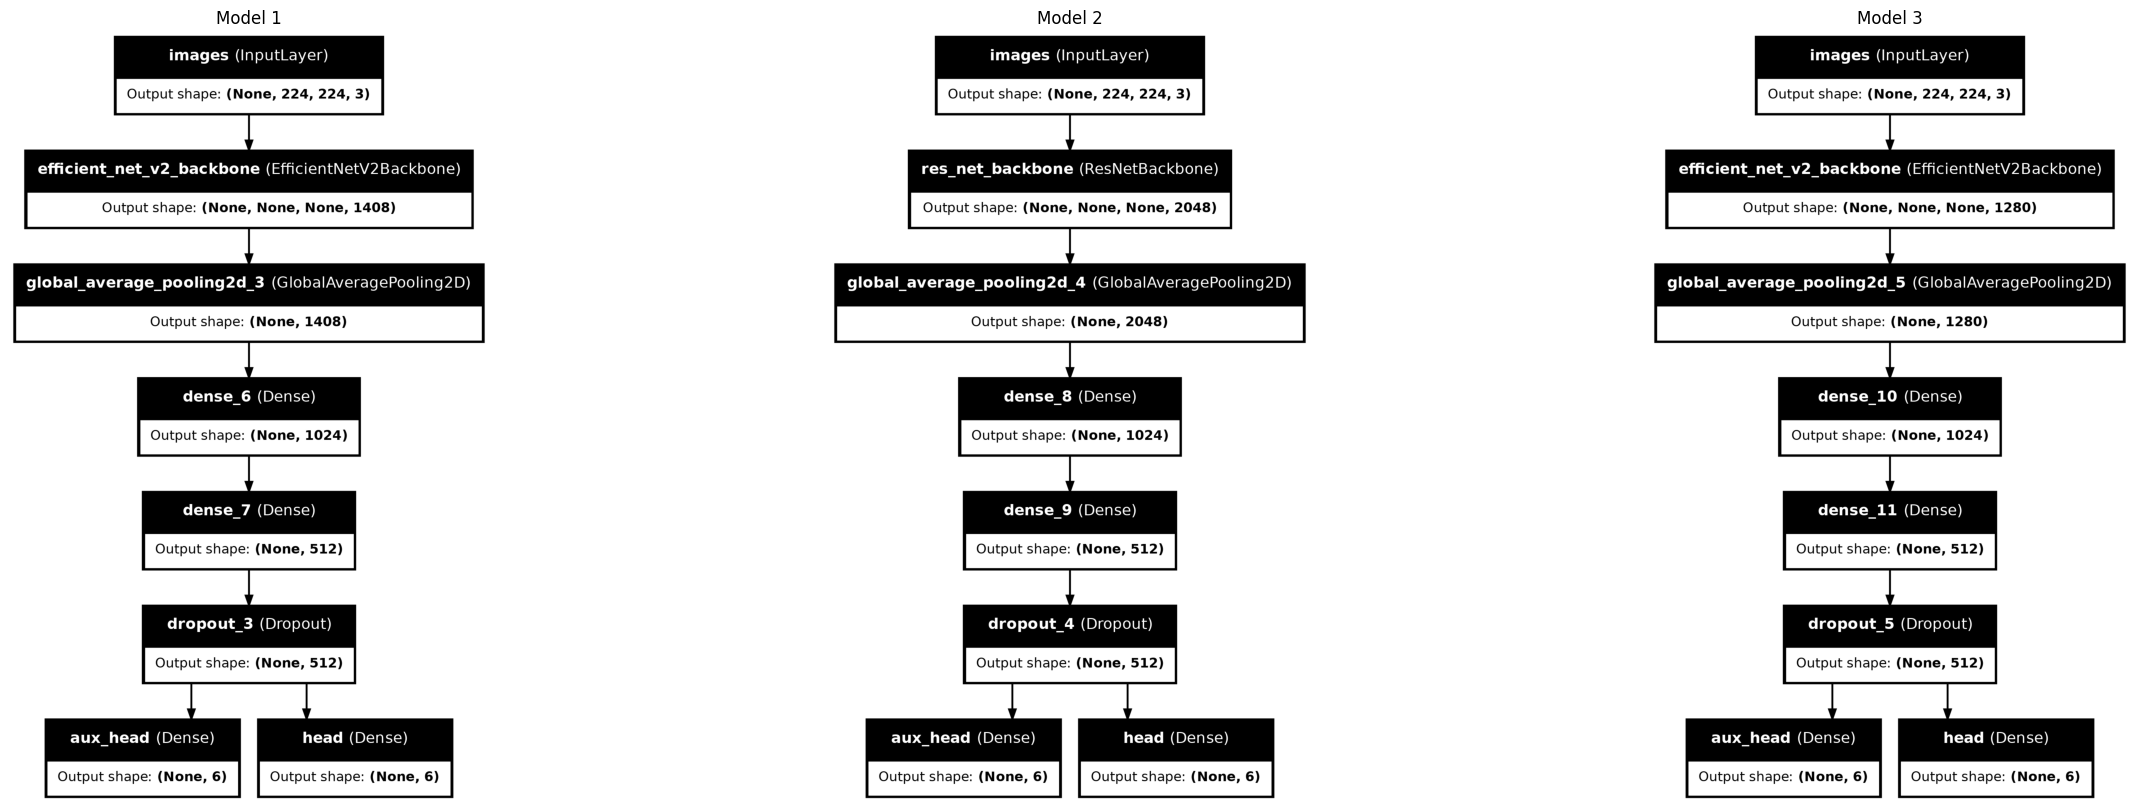
\includegraphics[width=1\textwidth]{assets/different_models.png}
    \caption{Visual overview of the 3 models with different backbones}
    \label{fig:models_overview}
\end{figure}

\subsubsection{Image CNN tuning}

% model x had the best loss in the end 
Looking at the results in \ref{fig:different_backbones} of the inital choice of hyperparameters for the different models the first thing we noticed was similar behavior of all the $R^2$ values in terms of their sign. The coefficient of determination is defined as follows 

\[
    R^2 = 1 - \frac{\sum_{i=1}^{n} (y_i - \hat{y}_i)^2}{\sum_{i=1}^{n} (y_i - \bar{y})^2} = 1 - \frac{SS_{res}}{SS_{tot}}  
\]
Where $SS_{res}$ is the residual sum of squares and $SS_{tot}$ is the total sum of squares. One observation in our results was that for all instances we had a negative $R^2$, implying that $SS_{res} > SS_{tot}$ meaning our model preforms worse than the baseline at $SS_{res} = SS_{tot}$. This is a clear indication that the model is fitting against the data, numerious reasons could be the cause of this. Due to the results of the intial training not being conclusive in regards to which model is better we decided to to simply continue with the model using the \textit{efficientnetv2\_b2\_imagenet} backbone as it has a high top 5 accuracy while also having fewer parameters.

\begin{figure}[!h]
    \centering
    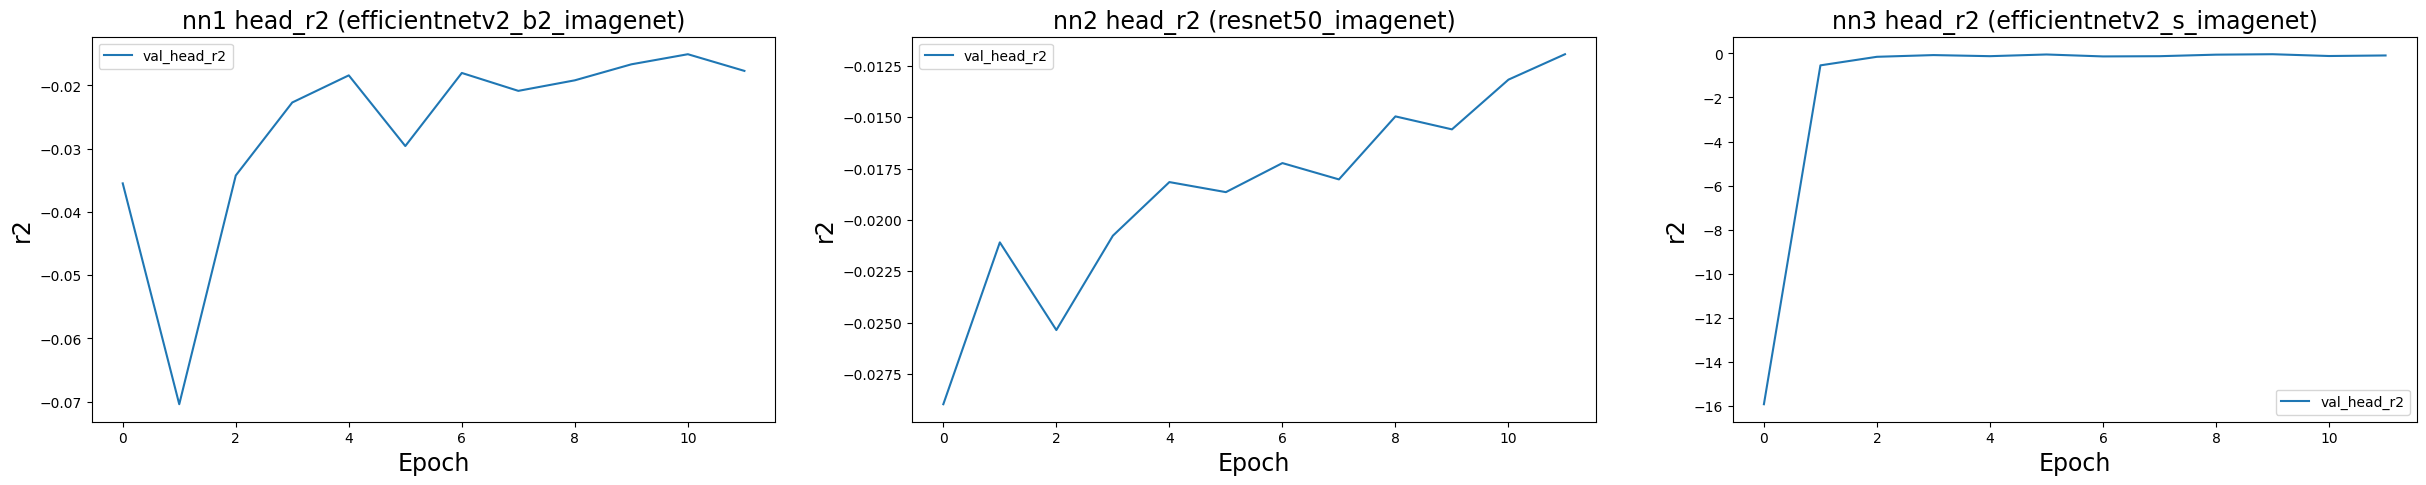
\includegraphics[width=1\textwidth]{assets/different_backbones.png}
    \caption{Validation loss for primary task with different backbones}
    \label{fig:different_backbones}
\end{figure}

While both of the EfficientNet backbones exhibit a similar behavior as they come from the same family of models; this being a fast convergence though also an early plateu at a more suboptimal loss. The ResNet50 backbone on the other hand has a slower convergence, but a more consisestent decrease in loss (increase in $R^2$). This could indicate that the ResNet50 backbone has a greater potential to learn from the data albeit in a slower manner. 

\smallskip 
One of the first things we decided to test was the learning rate schedule. We tested out 3 different schedules: step-based (baseline), exponential, and cosine annealing. The results demonstrated in \ref{fig:lr_schedules} show that the cosine annealing and exponential schedule had a slower convergence than the step-based schedule and a more erratic behavior.  

\begin{figure}[!h]
    \centering
    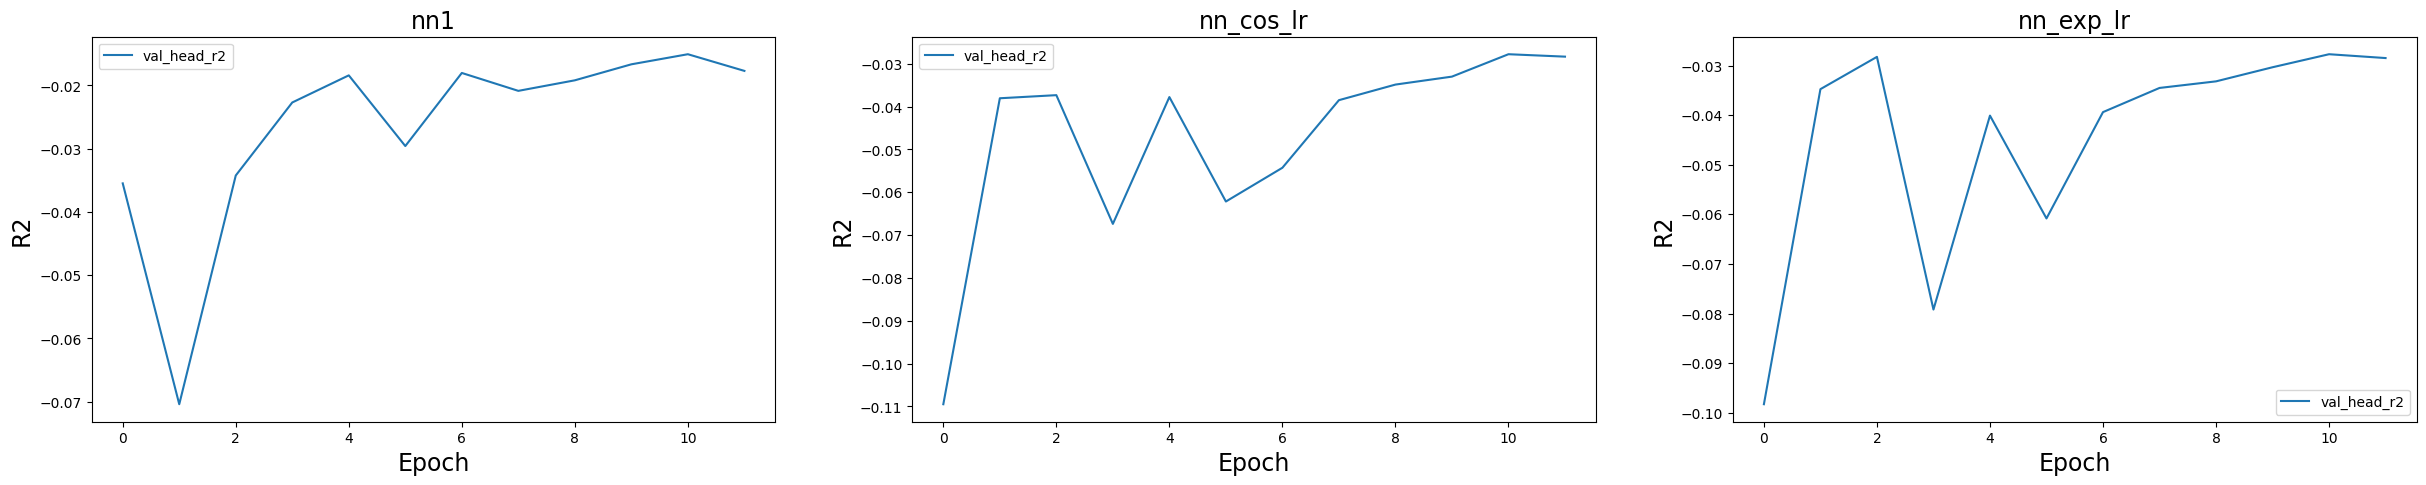
\includegraphics[width=0.4\textwidth]{assets/lr_schedule_diffs.png}
    \caption{Comparison of different learning rate schedules}
    \label{fig:lr_schedules}
\end{figure}

% we wanted to test out : different lr, backbone training on vs off 
    % test out cosine annealing 
    % test out exp 
    % plot step vs exp vs cosine annealing

Another point of consideration we had was the training of the backbone. We wanted to test out whether there was any difference in $R^2$ whether we allowed the model to adapt the weights of the backbone or not. The results of this can be seen in \ref{fig:backbone_training} in both of these instances we see the model converging at around the 2nd epoch and hitting a plateu of $\approx -0.03 R^2$. This is likely due to the fact that that the backbone requires little additional training to learn the features from the data and generalizes well to this task.

    % test out backbone training off for best lr schedule 
    % test out backbone training on for best lr schedule

\begin{figure}[!h]
    \centering
    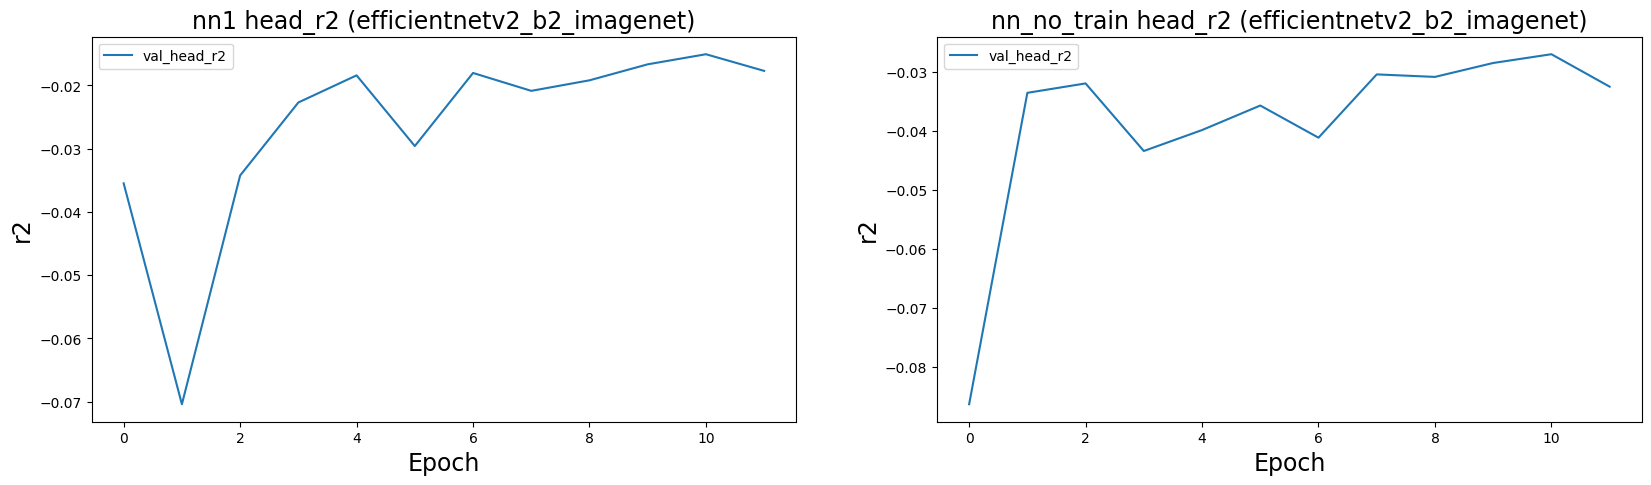
\includegraphics[width=0.7\textwidth]{assets/train_vs_notrain.png}
    \caption{Comparison of models with backbone training on (right) and off (left)}
    \label{fig:backbone_training}
\end{figure}

\subsubsection{CNN trained on images and geodata}

To construct the CNN trained on images and geodata we first created the two branches of the model, one to take in the image data and reduce it to a 1-tensor and similarly one to extract features from the tabular data. The two branches where then concatenated and fed to the main and auixallary task dense output layers. As the only difference here is the additional branch for the geodata we kept the hyperparameters the same to get a fair comparison between both approaches. A visual overview of the model can be seen in \ref{fig:geodata_model}.

\begin{figure}[!h]
    \centering 
    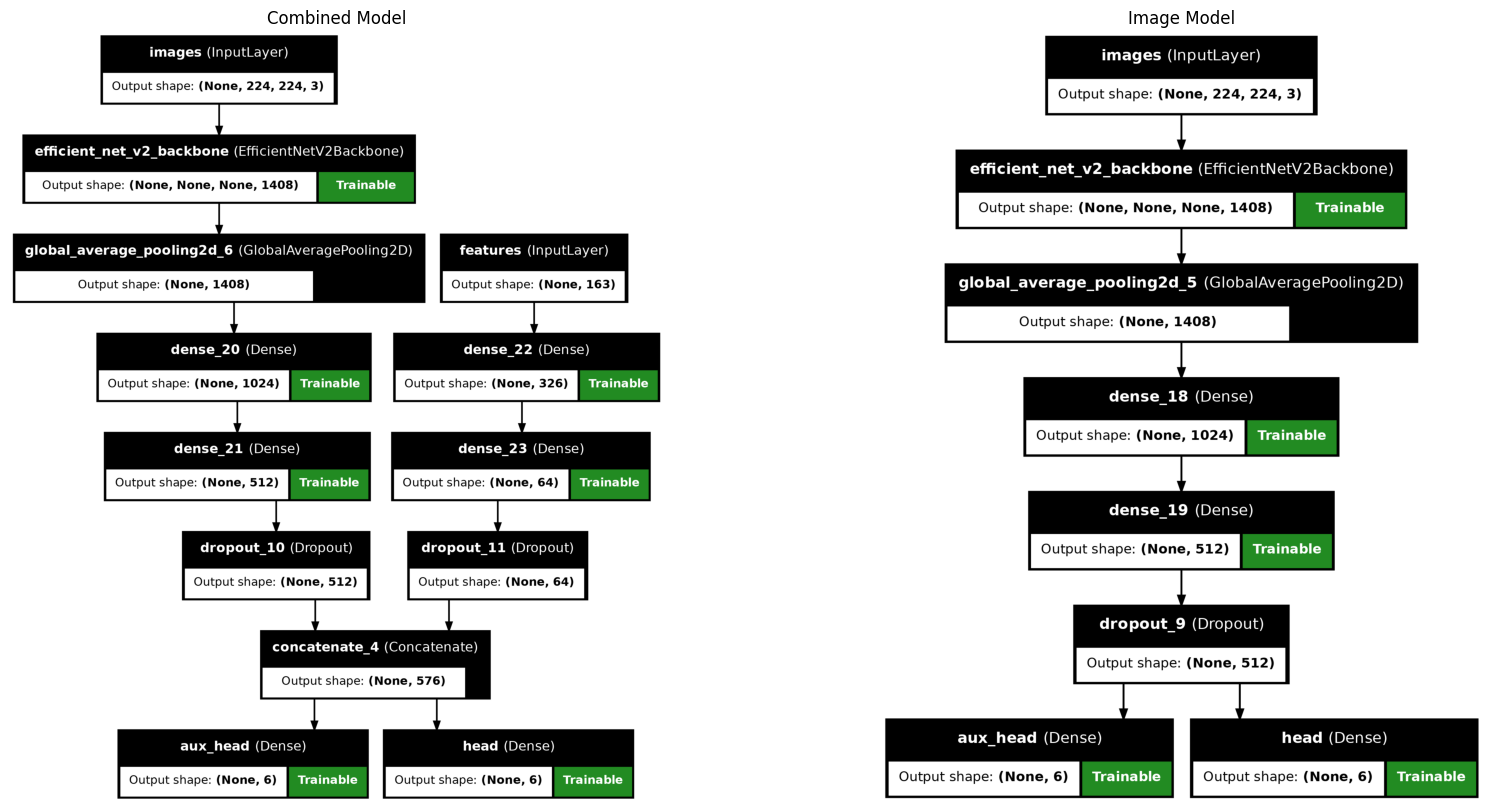
\includegraphics[width=0.8\textwidth]{assets/img_geo_model.png}
    \caption{(right) Model architecture of the CNN trained on images and geodata; (left) Model architecture of the CNN trained on images alone}
    \label{fig:geodata_model}
\end{figure}

% give an overview of the model
    % mention mainly the geodata model 
    % show a plot of the model

\subsection{Model comparative evaluation}

% evaluation of individual models 

For the final comparison we first looked at the basic evaluation metrics of either model. The results of this can be seen in \ref{fig:basic_evaluation}. We can see that the model trained on images and geodata has a higher $R^2$ suggesting a relative improvement in the prediction capability over just the image model which has a best recorded $R^2$ of <number>. 

\begin{figure}[!h]
    \centering
    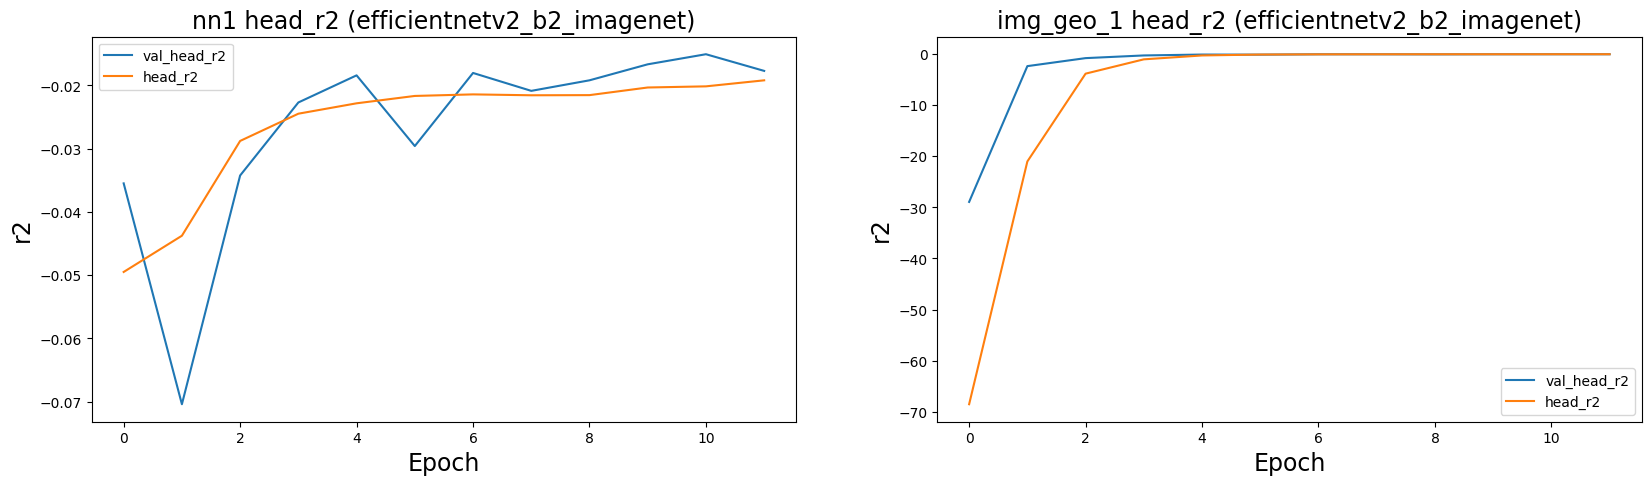
\includegraphics[width=0.7\textwidth]{assets/fin_img_vs_geo.png}
    \caption{Basic evaluation metrics of the two models}
    \label{fig:basic_evaluation}
\end{figure}

\smallskip

% comparative evaluation

\section{Results}

% give a simple summary of the results
One potential reason why the combined model performs better is simply that certain patterns are easier to learn from the geodata than from the images. Take the trait \textit{Stem specific density} for example, this is a trait that is likely to be more defined as a function of the environment \cite{plants8030065} rather than any visual cues. The same applies to the trait \textit{Leaf nitrogen content} which has been shown to be associated with abiotic stress (e.g. heat, cold, drought, etc.) \cite{Ye2022} and thus is likely to be more easily learned from the geodata.


\section{Discussion}

% discuss the results
The prediction of plant traits from images and geodata is a complex task that requires a CNN to learn and extract featues from both images and geodata. The results of our work show that a CNN trained on just image outpreforms one trained on images and geodata. Though neither of the models elaborated here is necessarily a good predictior, one of the main reasons for this is likely the complexity and nuance of the task. We now propose various directions for future work to improve the prediction capabilities of the models.

Hyperparameter tuning is one of the most important aspects of training a machine learning model. In our work we only tested a few different learning rate schedules and backbones. Random search - which as been demonstrated to be more effective than grid search \cite{JMLR:v13:bergstra12a} - would likely have been a better choice, albeit more computationally expensive. In addition we predominantly looked at hyperparameters, but varying the model architecture could have also been a benifical direction. A larger model could potentially learn more nuanced features in the data.

The training data itself can also be possibly modified to improve the model. Certain plant traits rely on some sense of relative scale to be elicited accurately (e.g. we know that a tree is bigger than flower regardless of image angle), this scale is easily lost due to the variability in how people take photos. One way of mitigating this could be to incorporate scale normalization through Depth Estimation, previous work \cite{Ummenhofer_2017} demonstrated the ability to train CNNs on the DIODE (Dense Indoor/Outdoor DEpth) \cite{vasiljevic2019diode} dataset to estimate depth. The learned depth information of the images could be used then as a moderator to scale the images to a common scale possibly improving the prediction capabilities.

How adaptable pretrained models are to new tasks is also is also something that could be further explored. Kunze et al. \cite{kunze2017transfer} answered this question by looking at the weight difference distribution per layer early and late into training. What they found was that models trained on a similar task to the target domain only had a minor change in the weight distribution. This reasoning could possibly be applied to more accurately find the optimal backbone. Additionally the use of a pretrained model could be further explored by looking at the effect of the number of layers frozen during training. 

\section{Conclusion}
To conclude we noticed that first and foremost the task to predict pant traits is a hard one. It requires a careful consideration during every step of the process from understanding the data to how a neural network architecture will learn from it. From our results we observed that a model trained on images and ancillary geodata converges faster but does not necessarily have a higher $R^2$ than a model trained on images alone. In the final tests run these results were also observed with our image model having a higher $R^2$ than the combined model. Though both models still have a negative $R^2$ suggesting some core limitations in the models. Future work could look at the effect of different hyperparameters, model architectures, and data modifications to improve the prediction capabilities of the models.   

\printbibliography

\end{document}